\documentclass[]{tufte-book}

% ams
\usepackage{amssymb,amsmath}

\usepackage{ifxetex,ifluatex}
\usepackage{fixltx2e} % provides \textsubscript
\ifnum 0\ifxetex 1\fi\ifluatex 1\fi=0 % if pdftex
  \usepackage[T1]{fontenc}
  \usepackage[utf8]{inputenc}
\else % if luatex or xelatex
  \makeatletter
  \@ifpackageloaded{fontspec}{}{\usepackage{fontspec}}
  \makeatother
  \defaultfontfeatures{Ligatures=TeX,Scale=MatchLowercase}
  \makeatletter
  \@ifpackageloaded{soul}{
     \renewcommand\allcapsspacing[1]{{\addfontfeature{LetterSpace=15}#1}}
     \renewcommand\smallcapsspacing[1]{{\addfontfeature{LetterSpace=10}#1}}
   }{}
  \makeatother

\fi

% graphix
\usepackage{graphicx}
\setkeys{Gin}{width=\linewidth,totalheight=\textheight,keepaspectratio}

% booktabs
\usepackage{booktabs}

% url
\usepackage{url}

% hyperref
\usepackage{hyperref}

% units.
\usepackage{units}


\setcounter{secnumdepth}{2}

% citations
\usepackage{natbib}
\bibliographystyle{apalike}

% pandoc syntax highlighting
\usepackage{color}
\usepackage{fancyvrb}
\newcommand{\VerbBar}{|}
\newcommand{\VERB}{\Verb[commandchars=\\\{\}]}
\DefineVerbatimEnvironment{Highlighting}{Verbatim}{commandchars=\\\{\}}
% Add ',fontsize=\small' for more characters per line
\newenvironment{Shaded}{}{}
\newcommand{\AlertTok}[1]{\textcolor[rgb]{1.00,0.00,0.00}{\textbf{#1}}}
\newcommand{\AnnotationTok}[1]{\textcolor[rgb]{0.38,0.63,0.69}{\textbf{\textit{#1}}}}
\newcommand{\AttributeTok}[1]{\textcolor[rgb]{0.49,0.56,0.16}{#1}}
\newcommand{\BaseNTok}[1]{\textcolor[rgb]{0.25,0.63,0.44}{#1}}
\newcommand{\BuiltInTok}[1]{#1}
\newcommand{\CharTok}[1]{\textcolor[rgb]{0.25,0.44,0.63}{#1}}
\newcommand{\CommentTok}[1]{\textcolor[rgb]{0.38,0.63,0.69}{\textit{#1}}}
\newcommand{\CommentVarTok}[1]{\textcolor[rgb]{0.38,0.63,0.69}{\textbf{\textit{#1}}}}
\newcommand{\ConstantTok}[1]{\textcolor[rgb]{0.53,0.00,0.00}{#1}}
\newcommand{\ControlFlowTok}[1]{\textcolor[rgb]{0.00,0.44,0.13}{\textbf{#1}}}
\newcommand{\DataTypeTok}[1]{\textcolor[rgb]{0.56,0.13,0.00}{#1}}
\newcommand{\DecValTok}[1]{\textcolor[rgb]{0.25,0.63,0.44}{#1}}
\newcommand{\DocumentationTok}[1]{\textcolor[rgb]{0.73,0.13,0.13}{\textit{#1}}}
\newcommand{\ErrorTok}[1]{\textcolor[rgb]{1.00,0.00,0.00}{\textbf{#1}}}
\newcommand{\ExtensionTok}[1]{#1}
\newcommand{\FloatTok}[1]{\textcolor[rgb]{0.25,0.63,0.44}{#1}}
\newcommand{\FunctionTok}[1]{\textcolor[rgb]{0.02,0.16,0.49}{#1}}
\newcommand{\ImportTok}[1]{#1}
\newcommand{\InformationTok}[1]{\textcolor[rgb]{0.38,0.63,0.69}{\textbf{\textit{#1}}}}
\newcommand{\KeywordTok}[1]{\textcolor[rgb]{0.00,0.44,0.13}{\textbf{#1}}}
\newcommand{\NormalTok}[1]{#1}
\newcommand{\OperatorTok}[1]{\textcolor[rgb]{0.40,0.40,0.40}{#1}}
\newcommand{\OtherTok}[1]{\textcolor[rgb]{0.00,0.44,0.13}{#1}}
\newcommand{\PreprocessorTok}[1]{\textcolor[rgb]{0.74,0.48,0.00}{#1}}
\newcommand{\RegionMarkerTok}[1]{#1}
\newcommand{\SpecialCharTok}[1]{\textcolor[rgb]{0.25,0.44,0.63}{#1}}
\newcommand{\SpecialStringTok}[1]{\textcolor[rgb]{0.73,0.40,0.53}{#1}}
\newcommand{\StringTok}[1]{\textcolor[rgb]{0.25,0.44,0.63}{#1}}
\newcommand{\VariableTok}[1]{\textcolor[rgb]{0.10,0.09,0.49}{#1}}
\newcommand{\VerbatimStringTok}[1]{\textcolor[rgb]{0.25,0.44,0.63}{#1}}
\newcommand{\WarningTok}[1]{\textcolor[rgb]{0.38,0.63,0.69}{\textbf{\textit{#1}}}}

% longtable
\usepackage{longtable,booktabs}

% multiplecol
\usepackage{multicol}

% strikeout
\usepackage[normalem]{ulem}

% morefloats
\usepackage{morefloats}


% tightlist macro required by pandoc >= 1.14
\providecommand{\tightlist}{%
  \setlength{\itemsep}{0pt}\setlength{\parskip}{0pt}}

% title / author / date
\title{Phân tích số liệu cơ bản}
\author{Phùng Khánh Lâm, Ong Phúc Thịnh}
\date{2019-07-10}

\usepackage{booktabs}
\usepackage{amsthm}
\makeatletter
\def\thm@space@setup{%
  \thm@preskip=8pt plus 2pt minus 4pt
  \thm@postskip=\thm@preskip
}
\makeatother

\begin{document}

\maketitle



{
\setcounter{tocdepth}{1}
\tableofcontents
}

\hypertarget{li-noi-u}{%
\chapter*{Lời nói đầu}\label{li-noi-u}}
\addcontentsline{toc}{chapter}{Lời nói đầu}

Test

\hypertarget{ni-dung-d-kin}{%
\section{Nội dung dự kiến}\label{ni-dung-d-kin}}

\begin{itemize}
\tightlist
\item
  Vì sao có cuốn sách này?
\item
  Mục tiêu
\item
  Đối tượng
\item
  Phương pháp:

  \begin{itemize}
  \tightlist
  \item
    Lý thuyết kết hợp với ví dụ thực tế
  \item
    Thực hành: R commander
  \end{itemize}
\item
  Đóng góp của nhóm tác giả
\end{itemize}

\hypertarget{d-liu-s-dung-trong-sach}{%
\section{Dữ liệu sử dụng trong sách}\label{d-liu-s-dung-trong-sach}}

Để minh hoạ cho các nội dung được trình bày, chúng tôi sử dụng các ví dụ thực tế, được phân tích bằng phần mềm R, trên bộ dữ liệu của một đoàn hệ tiền cứu trên trẻ nhập viện với chẩn đoán lâm sàng là sốt xuất huyết tại Bệnh viện Bệnh Nhiệt đới TP HCM từ năm 2001 đến năm 2009. Bộ dữ liệu này được công bố cùng với bài báo trình bày kết quả phân tích của nghiên cứu này \citep{Lam_2017}. Truy cập website của bài báo \url{https://journals.plos.org/plosntds/article?id=10.1371/journal.pntd.0005498} để tải về bộ dữ liệu này.

\hypertarget{intro}{%
\chapter{Giới thiệu về phân tích dữ liệu}\label{intro}}

Phân tích dữ liệu có thể được chia làm hai giai đoạn chính:

\begin{itemize}
\tightlist
\item
  Giai đoạn ban đầu: bao gồm hai giai đoạn nhỏ:

  \begin{itemize}
  \tightlist
  \item
    Kiểm tra và làm sạch số liệu
  \item
    Chuẩn bị dữ liệu cho phân tích
  \end{itemize}
\item
  Giai đoạn phân tích thực sự
\end{itemize}

You can label chapter and section titles using \texttt{\{\#label\}} after them, e.g., we can reference Chapter \ref{intro}. If you do not manually label them, there will be automatic labels anyway, e.g., Chapter \ref{methods}.

Figures and tables with captions will be placed in \texttt{figure} and \texttt{table} environments, respectively.

\begin{Shaded}
\begin{Highlighting}[]
\KeywordTok{par}\NormalTok{(}\DataTypeTok{mar =} \KeywordTok{c}\NormalTok{(}\DecValTok{4}\NormalTok{, }\DecValTok{4}\NormalTok{, }\FloatTok{0.1}\NormalTok{, }\FloatTok{0.1}\NormalTok{))}
\KeywordTok{plot}\NormalTok{(pressure, }\DataTypeTok{type =} \StringTok{"b"}\NormalTok{, }\DataTypeTok{pch =} \DecValTok{19}\NormalTok{)}
\end{Highlighting}
\end{Shaded}

\begin{figure}

{\centering 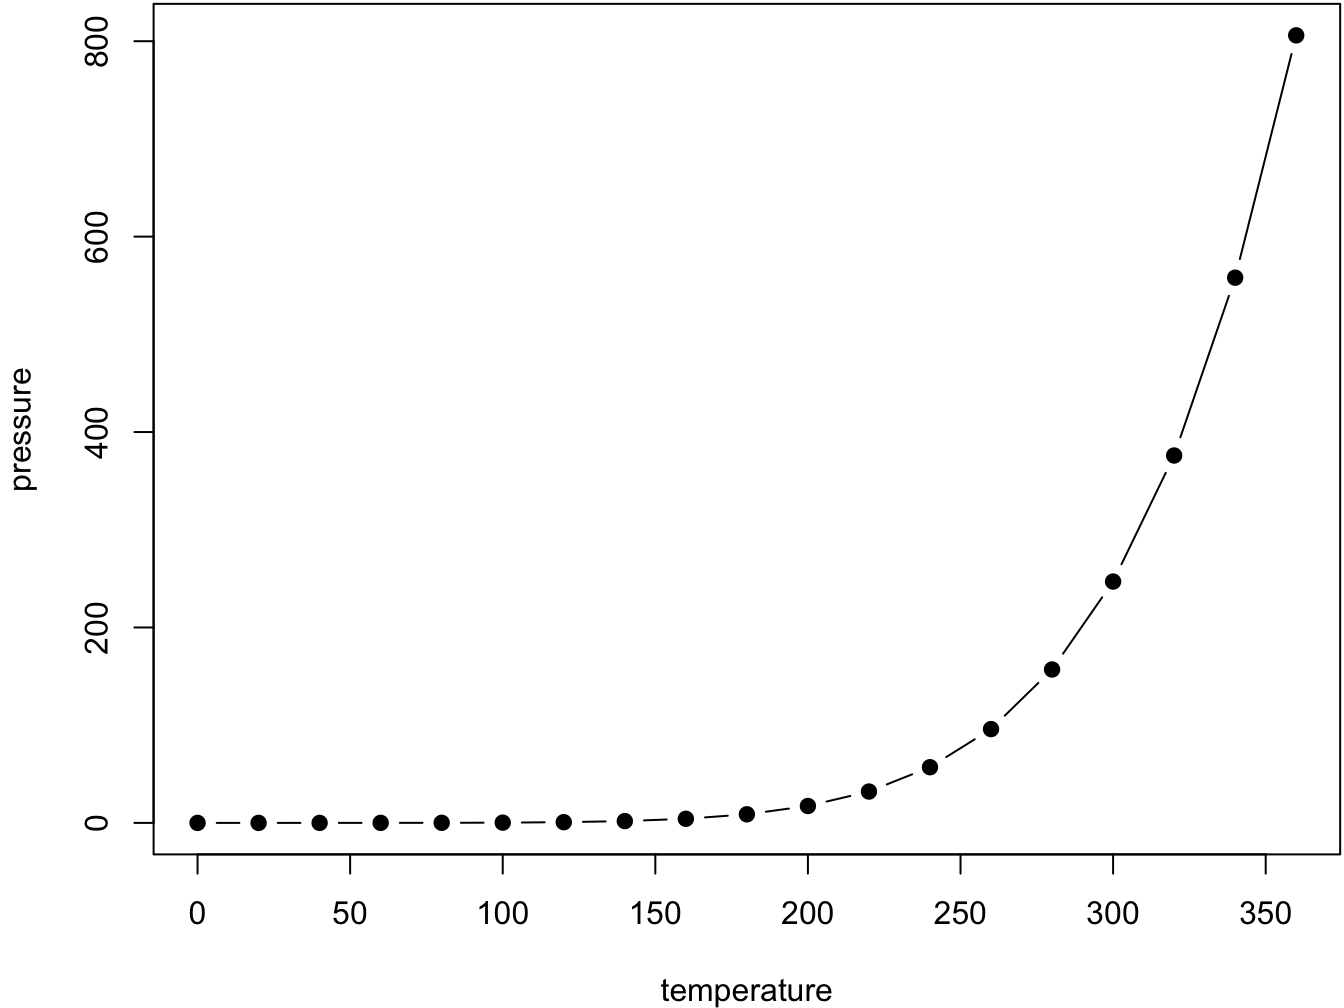
\includegraphics[width=0.8\linewidth]{book_da_basic_files/figure-latex/nice-fig-1} 

}

\caption[Here is a nice figure!]{Here is a nice figure!}\label{fig:nice-fig}
\end{figure}

Reference a figure by its code chunk label with the \texttt{fig:} prefix, e.g., see Figure \ref{fig:nice-fig}. Similarly, you can reference tables generated from \texttt{knitr::kable()}, e.g., see Table \ref{tab:nice-tab}.

\begin{Shaded}
\begin{Highlighting}[]
\NormalTok{knitr}\OperatorTok{::}\KeywordTok{kable}\NormalTok{(}
  \KeywordTok{head}\NormalTok{(iris, }\DecValTok{20}\NormalTok{), }\DataTypeTok{caption =} \StringTok{'Here is a nice table!'}\NormalTok{,}
  \DataTypeTok{booktabs =} \OtherTok{TRUE}
\NormalTok{)}
\end{Highlighting}
\end{Shaded}

\begin{table}[t]

\caption{\label{tab:nice-tab}Here is a nice table!}
\centering
\begin{tabular}{rrrrl}
\toprule
Sepal.Length & Sepal.Width & Petal.Length & Petal.Width & Species\\
\midrule
5.1 & 3.5 & 1.4 & 0.2 & setosa\\
4.9 & 3.0 & 1.4 & 0.2 & setosa\\
4.7 & 3.2 & 1.3 & 0.2 & setosa\\
4.6 & 3.1 & 1.5 & 0.2 & setosa\\
5.0 & 3.6 & 1.4 & 0.2 & setosa\\
\addlinespace
5.4 & 3.9 & 1.7 & 0.4 & setosa\\
4.6 & 3.4 & 1.4 & 0.3 & setosa\\
5.0 & 3.4 & 1.5 & 0.2 & setosa\\
4.4 & 2.9 & 1.4 & 0.2 & setosa\\
4.9 & 3.1 & 1.5 & 0.1 & setosa\\
\addlinespace
5.4 & 3.7 & 1.5 & 0.2 & setosa\\
4.8 & 3.4 & 1.6 & 0.2 & setosa\\
4.8 & 3.0 & 1.4 & 0.1 & setosa\\
4.3 & 3.0 & 1.1 & 0.1 & setosa\\
5.8 & 4.0 & 1.2 & 0.2 & setosa\\
\addlinespace
5.7 & 4.4 & 1.5 & 0.4 & setosa\\
5.4 & 3.9 & 1.3 & 0.4 & setosa\\
5.1 & 3.5 & 1.4 & 0.3 & setosa\\
5.7 & 3.8 & 1.7 & 0.3 & setosa\\
5.1 & 3.8 & 1.5 & 0.3 & setosa\\
\bottomrule
\end{tabular}
\end{table}

You can write citations, too. For example, we are using the \textbf{bookdown} package \citep{R-bookdown} in this sample book, which was built on top of R Markdown and \textbf{knitr} \citep{xie2015}.

\hypertarget{data_cleaning}{%
\chapter{Kiểm tra và làm sạch dữ liệu}\label{data_cleaning}}

Đây là bước đầu tiên nên được thực hiện khi nhận được một bộ số liệu, với mục tiêu là xây dựng được bộ số liệu sạch cho phân tích.

Sai sót hoặc dữ liệu bất thường rất thường gặp. Những sai sót này có thể bắt nguồn từ những sai sót trong quá trình thu thập dữ liệu và/hoặc quá trình nhập liệu. Một số lỗi có thể tình cờ phát hiện được trong khi phân tích, nhưng nhiều trường hợp không thể dễ dàng phát hiện và sẽ ảnh hưởng đến kết quả phân tích, thậm chí dẫn đến các sai sót trầm trọng. Vì vậy trước khi phân tích cần phải kiểm tra tính chính xác của số liệu để đảm bảo kết quả phân tích là chính xác nhất có thể.

\begin{table}[t]

\caption{\label{tab:UncleanedDataset}Dữ liệu chưa được làm sạch}
\centering
\begin{tabular}{llllrr}
\toprule
id & ngaysinh & ngaync & gioitinh & hct0 & cannang\_kg\\
\midrule
001 & 2013-05-08 & NA & 1 & 49 & 10\\
002 & 2018-12-03 & 2018-02-03 & Nữ & 250 & 50\\
003 & 2013-12-20 & 2018-12-13 & Nam & 50 & 20\\
003 & 2013-12-20 & 2018-12-13 & Nam & 50 & 20\\
\bottomrule
\end{tabular}
\end{table}

\hypertarget{error}{%
\section{Các nhóm lỗi dữ liệu thường gặp}\label{error}}

Rất nhiều lỗi khác nhau có thể gặp trong dữ liệu. Tuy nhiên, có thể tóm lại thành 4 nhóm lỗi thường gặp chính:

\begin{itemize}
\item
  Dữ liệu bị thiếu/mất (missing data): khi không có dữ liệu như mong đợi, có thể do trục trặc khi thu thập dữ liệu (đối tượng nghiên cứu bỏ nghiên cứu giữa chừng/không cung cấp thông tin, nghiên cứu viên quên thu thập thông tin) hoặc khi nhập liệu (nhập liệu sót, đặc biệt với phiếu thu thập thông tin dạng nhảy câu). Trong bộ dữ liệu, dữ liệu bị thiếu/mất thường được thể hiện bằng khoảng trắng (blank) hoặc giá trị NA (not available), ví dụ như ở biến số \textbf{ngaync} của đối tượng \textbf{001} trong Bảng \ref{tab:UncleanedDataset}.
\item
  Dữ liệu bị lặp lại (duplicated data): khi dữ liệu từ một hay nhiều đối tượng bị lặp lại một hay nhiều lần, thường do sai sót trong quá trình nhập liệu. Trong bộ dữ liệu, dữ liệu bị lặp lại thể hiện bằng việc một hay nhiều hàng dữ liệu bị lặp lại. Ví dụ như trong Bảng \ref{tab:UncleanedDataset}, dữ liệu của đối tượng \textbf{003} bị lặp lại thêm một lần.
\item
  Giá trị không hợp lý (out-of-range/inappropriate data): khi dữ liệu có giá trị nằm ngoài giới hạn thông thường (quá lớn hay quá bé, gặp ở các biến số liên tục) hoặc ngoài các giá trị cho phép (gặp ở các biến số phân nhóm) hoặc không phù hợp với thuộc tính của biến số (lẽ ra là giá trị số nhưng dữ liệu được nhập lại là chữ hoặc ngược lại). Đây có thể là lỗi trong quá trình thu thập dữ liệu hoặc khi nhập liệu. Ví dụ như trong Bảng \ref{tab:UncleanedDataset}, dữ liệu về \textbf{gioitinh} của đối tượng \textbf{001} được ghi nhận là \textbf{1}, trong khi đây là biến số về giới tính, vốn chỉ có hai giá trị \textbf{Nữ} hoặc \textbf{Nam}.
\item
  Không tương hợp giữa các biến số (inconsistent data): khi dữ liệu có giá trị không phù hợp trong mối tương quan với các biến số khác trong bộ dữ liệu. Đây có thể là lỗi trong quá trình thu thập dữ liệu hoặc khi nhập liệu. Lỗi này khó phát hiện hơn so với các lỗi còn lại. Ví dụ như trong Bảng \ref{tab:UncleanedDataset}, đối tượng \textbf{002} có \textbf{ngaync} (ngày vào nghiên cứu) là 2018-02-03 (ngày 03 tháng 02 năm 2018) trong khi \textbf{ngaysinh} (ngày sinh) lại là 2018-12-03 (ngày 03 tháng 12 năm 2018), nghĩa là đối tượng tham gia nghiên cứu trước khi sinh.
\end{itemize}

\hypertarget{detectmethod}{%
\section{Phương pháp phát hiện lỗi}\label{detectmethod}}

Để phát hiện các lỗi đã nêu trên, chúng ta có thể sử dụng các công cụ của thống kê mô tả, qua các chỉ số thống kê mô tả và/hoặc các biểu đồ.

\hypertarget{d-liu-bi-thiumt}{%
\subsection{Dữ liệu bị thiếu/mất}\label{d-liu-bi-thiumt}}

Được phát hiện bằng cách mô tả số giá trị có trong bộ dữ liệu và so sánh với số giá trị mong đợi. Hiện nay, các phần mềm thống kê đều cho phép mô tả số giá trị bị thiếu/mất, nếu các giá trị này được mã hoá ở dạng mà các phần mềm thống kê hiểu (khoảng trắng, hoặc NA đối với R). Nếu trong giai đoạn nhập liệu, giá trị bị thiếu/mất được mã hoá theo cách khác (điền vào một giá trị nào đó, ví dụ 9, 99, 999) thì trước khi dùng phần mềm thống kê để mô tả dữ liệu, cần định dạng dữ liệu về dạng mà phần mềm thống kê hiểu.

Ở ví dụ về bộ dữ liệu trong Bảng \ref{tab:UncleanedDataset}, bằng phần mềm R, chúng ta có thể dùng lệnh \texttt{summary()} để mô tả dữ liệu. Kết quả được trình bày dưới đây cho thấy có một giá trị bị thiếu/mất (NA) ở biến số \textbf{ngaync}.

\begin{Shaded}
\begin{Highlighting}[]
\KeywordTok{summary}\NormalTok{(dat)}
\end{Highlighting}
\end{Shaded}

\begin{verbatim}
##    id          ngaysinh        ngaync 
##  001:1   2013-05-08:1   2018-02-03:1  
##  002:1   2013-12-20:2   2018-12-13:2  
##  003:2   2018-12-03:1   NA's      :1  
##                                       
##                                       
##                                       
##  gioitinh      hct0          cannang_kg  
##  1  :1    Min.   : 49.00   Min.   :10.0  
##  Nam:2    1st Qu.: 49.75   1st Qu.:17.5  
##  Nữ :1    Median : 50.00   Median :20.0  
##           Mean   : 99.75   Mean   :25.0  
##           3rd Qu.:100.00   3rd Qu.:27.5  
##           Max.   :250.00   Max.   :50.0
\end{verbatim}

\hypertarget{d-liu-bi-lp-lai}{%
\subsection{Dữ liệu bị lặp lại}\label{d-liu-bi-lp-lai}}

Được phát hiện bằng cách mô tả số giá trị có trong bộ dữ liệu và so sánh với số giá trị mong đợi. Lỗi này cũng có thể phát hiện bằng mắt thường khi đã xếp dữ liệu theo thứ tự của mã số nghiên cứu, hoặc mô tả biến số mã số nghiên cứu (xem số giá trị mã số nghiên cứu khác nhau). Ngoài ra, một số phần mềm thống kê có thể có câu lệnh để kiểm tra dữ liệu bị lặp lại.

Ở ví dụ về bộ dữ liệu trong Bảng \ref{tab:UncleanedDataset}, bằng phần mềm R, chúng ta có thể dùng các cách sau:

\begin{itemize}
\tightlist
\item
  Kiểm tra số hàng của bộ dữ liệu
\end{itemize}

\begin{Shaded}
\begin{Highlighting}[]
\KeywordTok{nrow}\NormalTok{(dat)}
\end{Highlighting}
\end{Shaded}

\begin{verbatim}
## [1] 4
\end{verbatim}

Có 3 đối tượng nhưng bộ dữ liệu có 4 hàng.

\begin{itemize}
\tightlist
\item
  Mô tả biến số mã số nghiên cứu (ví dụ dùng lệnh \texttt{describe()} trong package Hmisc)
\end{itemize}

\begin{Shaded}
\begin{Highlighting}[]
\NormalTok{Hmisc}\OperatorTok{::}\KeywordTok{describe}\NormalTok{(dat}\OperatorTok{$}\NormalTok{id)}
\end{Highlighting}
\end{Shaded}

\begin{verbatim}
## dat$id 
##        n  missing distinct 
##        4        0        3 
##                          
## Value         1    2    3
## Frequency     1    1    2
## Proportion 0.25 0.25 0.50
\end{verbatim}

Biến số \textbf{id} (mã số nghiên cứu) có 4 giá trị, nhưng chỉ có 3 giá trị khác nhau (nghĩa là có một giá trị bị lặp lại).

\begin{itemize}
\tightlist
\item
  Kiểm tra số đối tượng nghiên cứu bằng cách kiểm tra số giá trị mã số nghiên cứu khác nhau
\end{itemize}

\begin{Shaded}
\begin{Highlighting}[]
\KeywordTok{length}\NormalTok{(dat}\OperatorTok{$}\NormalTok{id)}
\end{Highlighting}
\end{Shaded}

\begin{verbatim}
## [1] 4
\end{verbatim}

\begin{Shaded}
\begin{Highlighting}[]
\KeywordTok{length}\NormalTok{(}\KeywordTok{unique}\NormalTok{(dat}\OperatorTok{$}\NormalTok{id))}
\end{Highlighting}
\end{Shaded}

\begin{verbatim}
## [1] 3
\end{verbatim}

Biến số \textbf{id} (mã số nghiên cứu) có 4 giá trị, nhưng chỉ có 3 giá trị khác nhau (nghĩa là có một giá trị bị lặp lại).

\begin{itemize}
\tightlist
\item
  Kiểm tra dữ liệu lặp lại bằng lệnh \texttt{anyDuplicated} hoặc \texttt{duplicated}
\end{itemize}

\begin{Shaded}
\begin{Highlighting}[]
\KeywordTok{anyDuplicated}\NormalTok{(dat)}
\end{Highlighting}
\end{Shaded}

\begin{verbatim}
## [1] 4
\end{verbatim}

\begin{Shaded}
\begin{Highlighting}[]
\KeywordTok{duplicated}\NormalTok{(dat)}
\end{Highlighting}
\end{Shaded}

\begin{verbatim}
## [1] FALSE FALSE FALSE  TRUE
\end{verbatim}

Dữ liệu ở hàng thứ 4 trong bộ dữ liệu \textbf{dat} là dữ liệu lặp lại.

\hypertarget{gia-tri-khong-hp-ly}{%
\subsection{Giá trị không hợp lý}\label{gia-tri-khong-hp-ly}}

Được phát hiện bằng cách mô tả tất cả các giá trị trong biến số bằng các chỉ số hoặc biểu đồ, từ đó tìm ra các giá trị khác biệt so với các giá trị còn lại của biến số.

Ở ví dụ về bộ dữ liệu trong Bảng \ref{tab:UncleanedDataset}, bằng phần mềm R, chúng ta có thể dùng các cách sau:

\begin{itemize}
\tightlist
\item
  Mô tả các giá trị khác nhau của biến số bằng lệnh \texttt{unique()} hoặc \texttt{table()} (chỉ thích hợp với biến số có ít giá trị khác nhau, ví dụ biến số phân nhóm)
\end{itemize}

\begin{Shaded}
\begin{Highlighting}[]
\KeywordTok{unique}\NormalTok{(dat}\OperatorTok{$}\NormalTok{gioitinh)}
\end{Highlighting}
\end{Shaded}

\begin{verbatim}
## [1] 1   Nữ  Nam
## Levels: 1 Nam Nữ
\end{verbatim}

\begin{Shaded}
\begin{Highlighting}[]
\KeywordTok{table}\NormalTok{(dat}\OperatorTok{$}\NormalTok{gioitinh)}
\end{Highlighting}
\end{Shaded}

\begin{verbatim}
## 
##   1 Nam  Nữ 
##   1   2   1
\end{verbatim}

Biến số \textbf{gioitinh} (giới tính) có 3 giá trị: 1, Nữ, Nam; trong đó giá trị \textbf{1} không phù hợp.

\begin{itemize}
\tightlist
\item
  Mô tả khoảng giá trị, giá trị nhỏ nhất, giá trị lớn nhất để tìm các giá trị quá lớn hoặc quá bé so với mong đợi
\end{itemize}

\begin{Shaded}
\begin{Highlighting}[]
\KeywordTok{summary}\NormalTok{(dat}\OperatorTok{$}\NormalTok{hct0)}
\end{Highlighting}
\end{Shaded}

\begin{verbatim}
##    Min. 1st Qu.  Median    Mean 3rd Qu. 
##   49.00   49.75   50.00   99.75  100.00 
##    Max. 
##  250.00
\end{verbatim}

\begin{Shaded}
\begin{Highlighting}[]
\KeywordTok{range}\NormalTok{(dat}\OperatorTok{$}\NormalTok{hct0)}
\end{Highlighting}
\end{Shaded}

\begin{verbatim}
## [1]  49 250
\end{verbatim}

\begin{Shaded}
\begin{Highlighting}[]
\KeywordTok{min}\NormalTok{(dat}\OperatorTok{$}\NormalTok{hct0)}
\end{Highlighting}
\end{Shaded}

\begin{verbatim}
## [1] 49
\end{verbatim}

\begin{Shaded}
\begin{Highlighting}[]
\KeywordTok{max}\NormalTok{(dat}\OperatorTok{$}\NormalTok{hct0)}
\end{Highlighting}
\end{Shaded}

\begin{verbatim}
## [1] 250
\end{verbatim}

Biến số \textbf{hct0} (dung tích hồng cầu ở thời điểm lúc mới vào nghiên cứu) có khoảng giá trị từ 49\% (giá trị nhỏ nhất) đến 250\% (giá trị lớn nhất), trong đó giá trị \textbf{250} là không phù hợp với giá trị mong đợi của dung tích hồng cầu.

\begin{itemize}
\tightlist
\item
  Mô tả giá trị bằng biểu đồ cột (với biến số phân nhóm)
\end{itemize}

\begin{Shaded}
\begin{Highlighting}[]
\KeywordTok{barplot}\NormalTok{(}\KeywordTok{table}\NormalTok{(dat}\OperatorTok{$}\NormalTok{gioitinh))}
\end{Highlighting}
\end{Shaded}

\begin{center}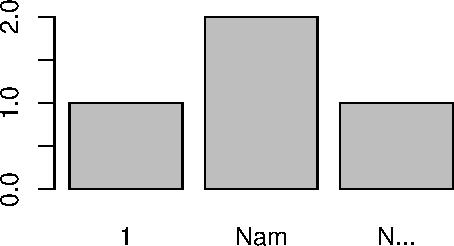
\includegraphics[width=0.8\linewidth]{book_da_basic_files/figure-latex/detectInappropriate3-1} \end{center}

Biến số \textbf{gioitinh} có giá trị \textbf{1}, không phù hợp với các giá trị còn lại.

\begin{itemize}
\tightlist
\item
  Mô tả giá trị bằng histogram hoặc boxplot (với biến số liên tục)
\end{itemize}

\begin{Shaded}
\begin{Highlighting}[]
\KeywordTok{hist}\NormalTok{(dat}\OperatorTok{$}\NormalTok{hct0)}
\end{Highlighting}
\end{Shaded}

\begin{center}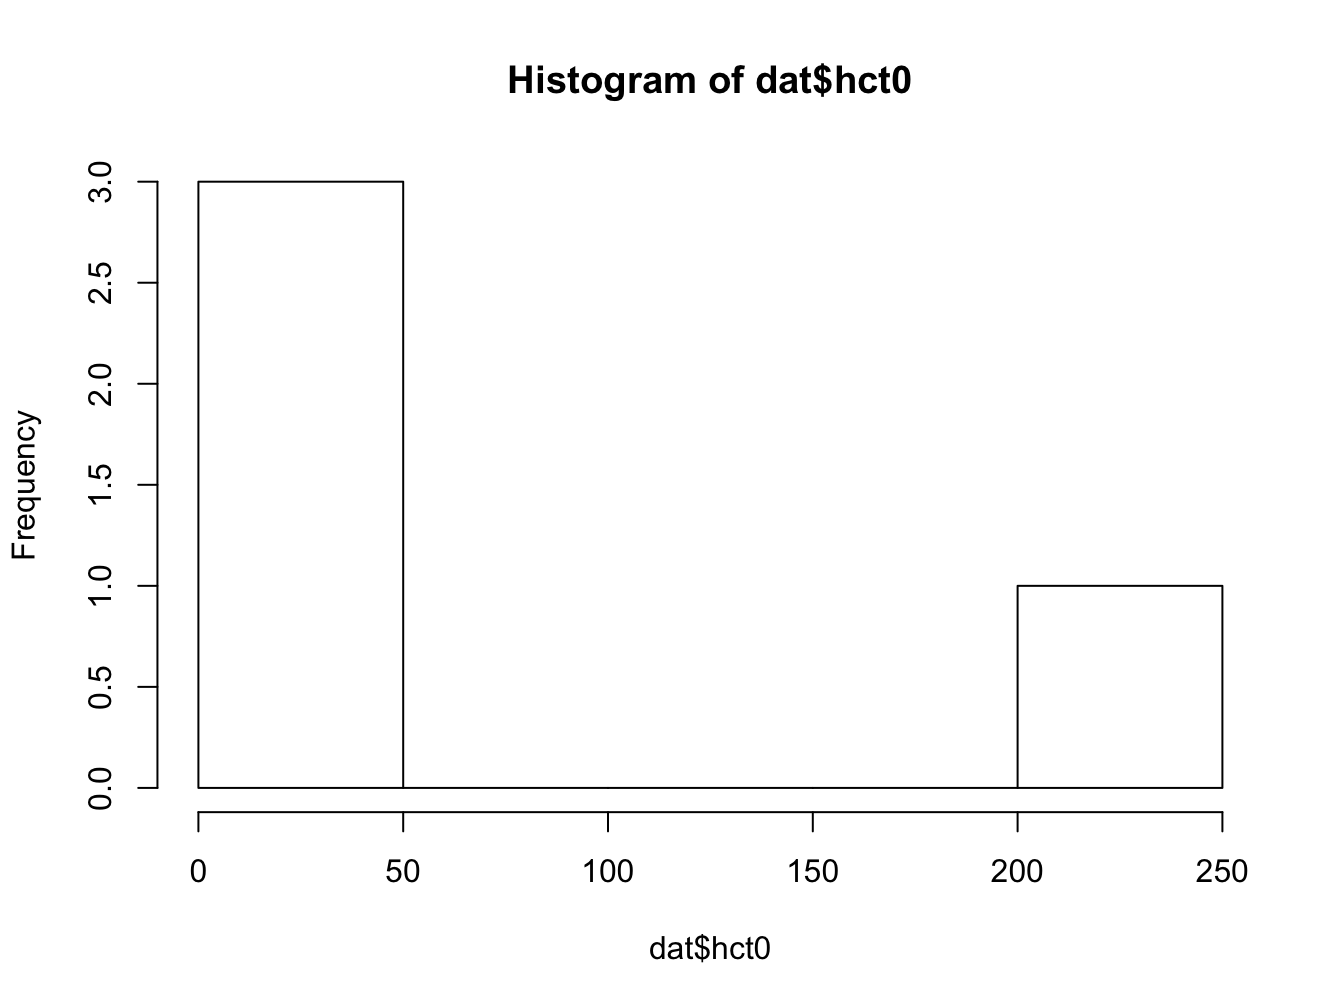
\includegraphics[width=0.8\linewidth]{book_da_basic_files/figure-latex/detectInappropriate4-1} \end{center}

\begin{Shaded}
\begin{Highlighting}[]
\KeywordTok{boxplot}\NormalTok{(dat}\OperatorTok{$}\NormalTok{hct0)}
\end{Highlighting}
\end{Shaded}

\begin{center}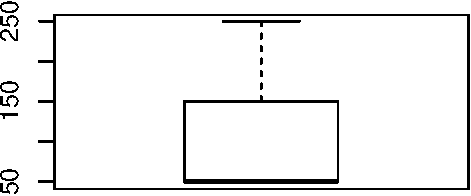
\includegraphics[width=0.8\linewidth]{book_da_basic_files/figure-latex/detectInappropriate4-2} \end{center}

Biến số \textbf{hct0} có giá trị \textbf{250}, rất khác biệt so với các giá trị còn lại và nằm ngoài khoảng giá trị mong đợi cho dung tích hồng cầu.

\hypertarget{khong-tuong-hp-gia-cac-bin-s}{%
\subsection{Không tương hợp giữa các biến số}\label{khong-tuong-hp-gia-cac-bin-s}}

Được phát hiện bằng cách mô tả biến số thứ cấp tạo ra từ các biến số liên quan, hoặc dùng biểu đồ mô tả mối liên hệ giữa hai biến số với nhau.

Ở ví dụ về bộ dữ liệu trong Bảng \ref{tab:UncleanedDataset}, bằng phần mềm R, chúng ta có thể dùng các cách sau:

\begin{itemize}
\tightlist
\item
  Mô tả biến số thứ cấp: ví dụ mô tả biến số \textbf{tuoi} (tuổi lúc vào nghiên cứu), được tính từ biến số \textbf{ngaysinh} và \textbf{ngaync}
\end{itemize}

\begin{Shaded}
\begin{Highlighting}[]
\NormalTok{dat}\OperatorTok{$}\NormalTok{tuoi <-}\StringTok{ }\KeywordTok{as.numeric}\NormalTok{(}\KeywordTok{difftime}\NormalTok{(}\KeywordTok{as.Date}\NormalTok{(dat}\OperatorTok{$}\NormalTok{ngaync), }
    \KeywordTok{as.Date}\NormalTok{(dat}\OperatorTok{$}\NormalTok{ngaysinh), }\DataTypeTok{units =} \StringTok{"days"}\NormalTok{))}
\KeywordTok{summary}\NormalTok{(dat}\OperatorTok{$}\NormalTok{tuoi)}
\end{Highlighting}
\end{Shaded}

\begin{verbatim}
##    Min. 1st Qu.  Median    Mean 3rd Qu. 
##    -303     758    1819    1112    1819 
##    Max.    NA's 
##    1819       1
\end{verbatim}

\begin{Shaded}
\begin{Highlighting}[]
\KeywordTok{boxplot}\NormalTok{(dat}\OperatorTok{$}\NormalTok{tuoi)}
\end{Highlighting}
\end{Shaded}

\begin{center}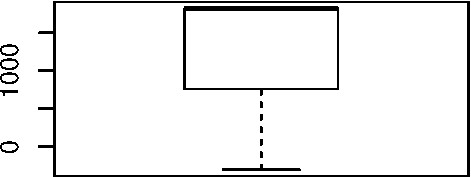
\includegraphics[width=0.8\linewidth]{book_da_basic_files/figure-latex/detectInconsistency1-1} \end{center}

Có một trường hợp \textbf{tuoi} (tuổi lúc vào nghiên cứu) \textless{} 0.

\begin{itemize}
\tightlist
\item
  Dùng biểu đồ mô tả mối liên hệ giữa hai biến số \textbf{ngaysinh} và \textbf{ngaync}
\end{itemize}

\begin{Shaded}
\begin{Highlighting}[]
\CommentTok{## phân tán đồ (scatterplot) của ngaysinh và}
\CommentTok{## ngaync}
\KeywordTok{plot}\NormalTok{(}\DataTypeTok{x =} \KeywordTok{as.Date}\NormalTok{(dat}\OperatorTok{$}\NormalTok{ngaysinh), }\DataTypeTok{y =} \KeywordTok{as.Date}\NormalTok{(dat}\OperatorTok{$}\NormalTok{ngaync))}
\CommentTok{## đường thẳng qua các điểm ngaysinh bằng}
\CommentTok{## ngaync}
\KeywordTok{abline}\NormalTok{(}\DataTypeTok{a =} \DecValTok{0}\NormalTok{, }\DataTypeTok{b =} \DecValTok{1}\NormalTok{)}
\end{Highlighting}
\end{Shaded}

\begin{center}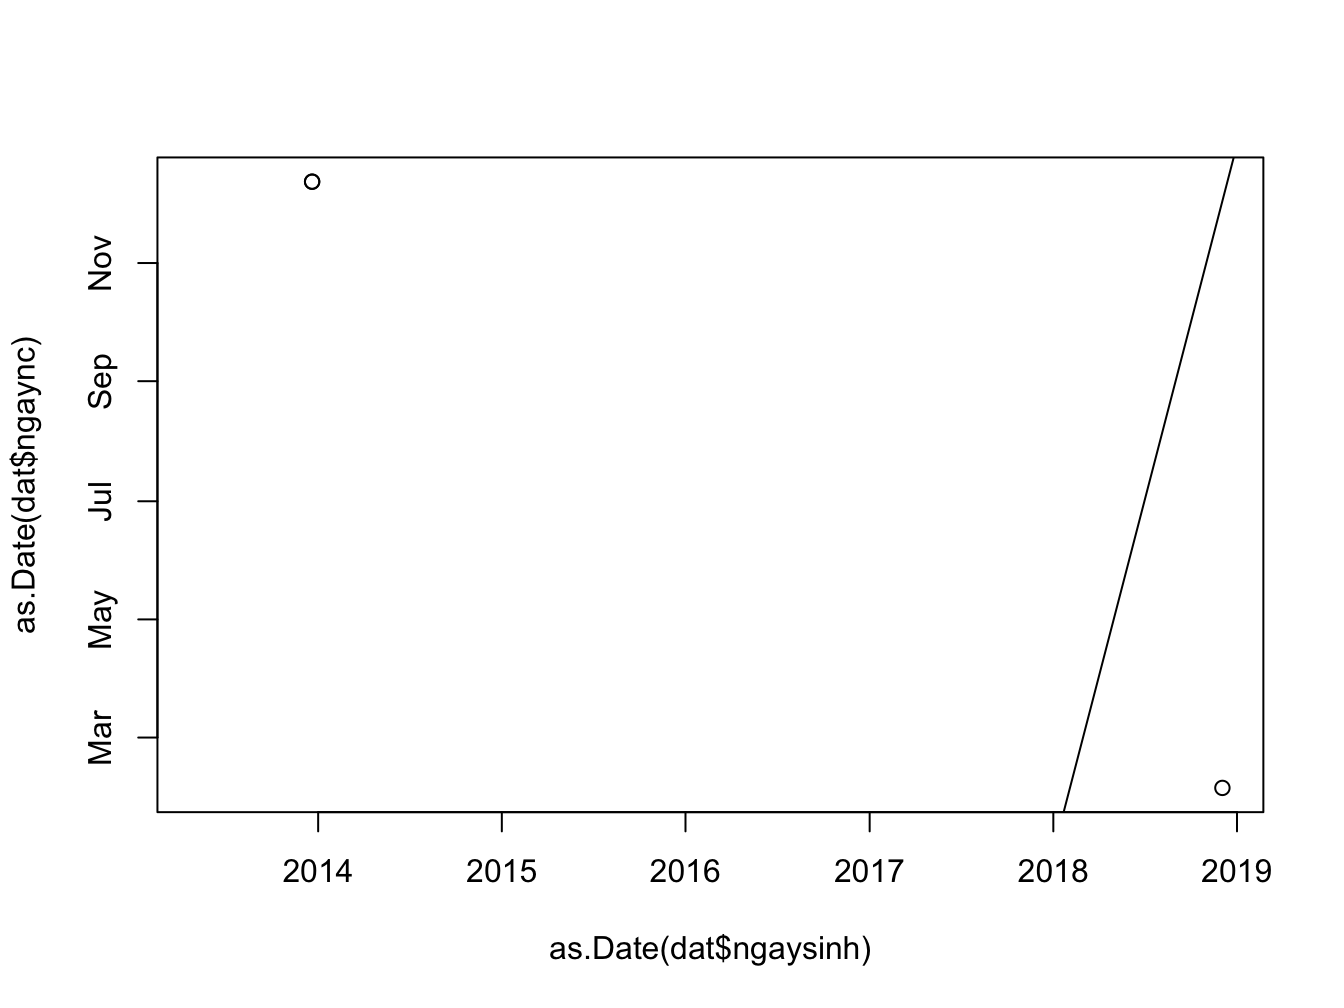
\includegraphics[width=0.8\linewidth]{book_da_basic_files/figure-latex/detectInconsistency2-1} \end{center}

Có một trường hợp \textbf{ngaync} nhỏ hơn \textbf{ngaysinh} (nằm phía dưới đường thẳng đi qua các giá trị \textbf{ngaync} bằng \textbf{ngaysinh}) trong khi mong đợi \textbf{ngaync} phải lớn hơn \textbf{ngaysinh} (đối tượng phải được sinh ra trước khi vào nghiên cứu).

\hypertarget{quy-trinh-kim-tra-va-lam-sach-d-liu}{%
\section{Quy trình kiểm tra và làm sạch dữ liệu}\label{quy-trinh-kim-tra-va-lam-sach-d-liu}}

Để phát hiện và loại bỏ tối đa các sai sót có thể có nhằm có được bộ dữ liệu sạch và đáng tin cậy cho phân tích, chúng ta cần kiểm tra và làm sạch dữ liệu một cách có hệ thống theo 3 bước như sau:

\hypertarget{tim-li}{%
\subsection{Tìm lỗi}\label{tim-li}}

Dựa vào các phương pháp thống kê mô tả (sử dụng chỉ số và/hoặc biểu đồ, như đã trình bày ở mục \ref{detectmethod}) để tìm các lỗi thường gặp (như đã trình bày ở mục \ref{error}).

Các lỗi tìm thấy nên được tổng hợp lại trong một file dữ liệu trước khi tiến hành bước tiếp theo. File dữ liệu này nên bao gồm các thông tin sau:

\begin{itemize}
\tightlist
\item
  Lỗi tìm thấy là gì? (loại lỗi)
\item
  Lỗi ở đâu? (biến số liên quan, mã số nghiên cứu liên quan)
\end{itemize}

\hypertarget{chn-oan-li}{%
\subsection{Chẩn đoán lỗi}\label{chn-oan-li}}

Trong bước này, chúng ta sẽ dựa vào kiến thức chuyên môn và hiểu biết về nghiên cứu và quá trình thu thập dữ liệu - nhập liệu trong nghiên cứu để đánh giá xem các lỗi tìm thấy trong dữ liệu có thực sự là lỗi hay không. Khi đánh giá, cần đối chiếu với dữ liệu gốc (dữ liệu thu thập trên phiếu thu thập bằng giấy) nếu có. Sau khi đánh giá, các lỗi này có thể được phân loại thành:

\begin{itemize}
\tightlist
\item
  Lỗi thực sự
\item
  Không phải lỗi (chỉ là giá trị hiếm gặp)
\item
  Không chắc: không thể xác định có phải là lỗi không dựa vào các thông tin hiện có
\end{itemize}

\hypertarget{sa-li-lam-sach-d-liu}{%
\subsection{Sửa lỗi (làm sạch dữ liệu)}\label{sa-li-lam-sach-d-liu}}

Tùy theo phân loại ở bước chẩn đoán lỗi, chúng ta sẽ có cách sửa lỗi phù hợp:

\begin{itemize}
\tightlist
\item
  Lỗi thực sự: sửa lại thành giá trị đúng (nếu có cơ sở cho giá trị đúng, ví dụ như giá trị gốc được lưu trên giấy) hoặc xoá hẳn giá trị sai (nếu không thể xác định được giá trị đúng).
\item
  Không phải lỗi: giữ nguyên, không thay đổi giá trị trong dữ liệu.
\item
  Không chắc: cân nhắc giữa giữ nguyên và xoá hẳn giá trị này.
\end{itemize}

Các bước trên và mọi thay đổi trong bộ dữ liệu nên được ghi nhận lại với các thông tin như:

\begin{itemize}
\tightlist
\item
  Lỗi tìm thấy là gì? (loại lỗi)
\item
  Lỗi ở đâu? (biến số liên quan, mã số nghiên cứu liên quan)
\item
  Chẩn đoán lỗi là gì?
\item
  Người chẩn đoán lỗi?
\item
  Quyết định đưa ra với lỗi?
\item
  Người đưa ra quyết định?
\item
  Nếu có sửa lỗi thì giá trị cũ là gì, giá trị mới là gì? người sửa lỗi? ngày sửa lỗi?
\end{itemize}

Vấn đề này đặc biệt quan trọng khi làm việc trong một nhóm và nhằm đảm bảo tính minh bạch và rõ ràng trong quản lý dữ liệu. Một ví dụ về file dữ liệu ghi nhận các bước liên quan đến việc kiểm tra và làm sạch dữ liệu như sau:

\begin{figure}

{\centering 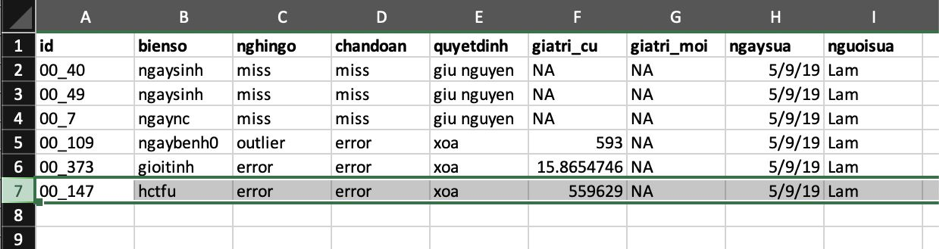
\includegraphics[width=0.8\linewidth]{figures/02_04} 

}

\caption[File ghi nhận việc kiểm tra và làm sạch dữ liệu]{File ghi nhận việc kiểm tra và làm sạch dữ liệu}\label{fig:documentclean}
\end{figure}

\hypertarget{chun-bi-d-liu-cho-phan-tich}{%
\chapter{Chuẩn bị dữ liệu cho phân tích}\label{chun-bi-d-liu-cho-phan-tich}}

Dữ liệu sau khi làm sạch có thể chưa phân tích được ngay, mà cần phải biến đổi để phù hợp với mục tiêu và kỹ thuật phân tích.

\hypertarget{tao-them-bin-s-mi}{%
\section{Tạo thêm biến số mới}\label{tao-them-bin-s-mi}}

Tạo thêm biến số mới dựa trên các biến số sẵn có: Ví dụ thu thập ngày tháng năm sinh, cần tạo thêm biến số là tuổi; hoặc thu thập cân nặng và chiều cao, cần tạo thêm biến BMI để phân tích.

\hypertarget{inh-dang-bin-s}{%
\section{Định dạng biến số}\label{inh-dang-bin-s}}

(phần này em không chắc là trình bày nội dung gì)

\hypertarget{chuyn-dang-d-liu-cho-phu-hp-vi-phan-tich}{%
\chapter{Chuyển dạng dữ liệu cho phù hợp với phân tích}\label{chuyn-dang-d-liu-cho-phu-hp-vi-phan-tich}}

\hypertarget{kt-hp-cac-bang-d-liu-vi-nhau}{%
\section{Kết hợp các bảng dữ liệu với nhau}\label{kt-hp-cac-bang-d-liu-vi-nhau}}

Dữ liệu có thể nằm ở nhiều tập tin khác nhau hoặc do nhiều người nhập liệu, cần phải ghép lại thành một bảng dữ liệu hoàn chỉnh để có đầy đủ thông tin phục vụ cho việc phân tích.

\hypertarget{d-liu-dang-dai-hay-dang-rng}{%
\section{Dữ liệu dạng dài hay dạng rộng}\label{d-liu-dang-dai-hay-dang-rng}}

Ví dụ ta có bảng dữ liệu như sau gồm 4 cột:

\begin{figure}
\centering
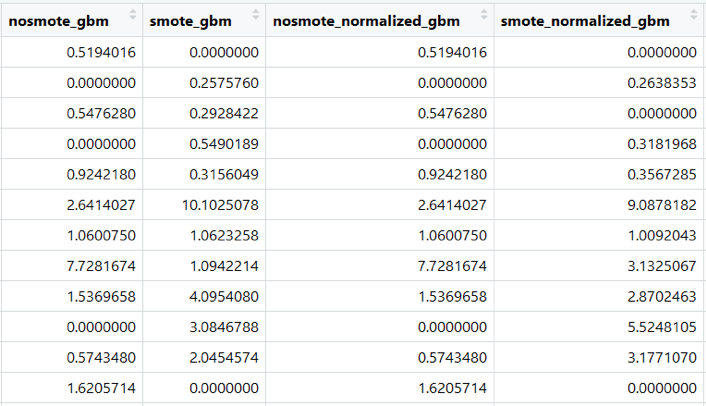
\includegraphics{figures/02_05.png}
\caption{Ví dụ về dữ liệu dạng rộng}
\end{figure}

Ta có thể biến đổi dữ liệu từ có 4 cột này thành chỉ có 2 cột như sau:

\begin{figure}
\centering
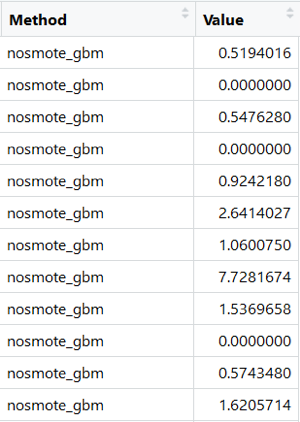
\includegraphics{figures/02_06.png}
\caption{Ví dụ về dữ liệu dạng dài}
\end{figure}

Các giá trị trong cột Method là nosmote\_gbm, smote\_gbm, nosmote\_normalized\_gbm, smote\_normalized\_gbm chính là tên của 4 cột ban đầu. Giá trị trong cột Value là những con số tương ứng với mỗi phương pháp trong Method. Việc biến đổi này không làm mất đi thông tin trong bộ dữ liệu mà chỉ làm thay đổi hình dạng trình bày thông tin. Dữ liệu to bè theo chiều ngang (gồm nhiều cột) gọi là dữ liệu dạng rộng (wide format). Dữ liệu sau khi biến đổi chỉ có 2 cột nhưng sẽ kéo dài xuống thành rất nhiều dòng gọi là dữ liệu dạng dài (long format).

\hypertarget{phan-tich-mo-ta}{%
\chapter{Phân tích mô tả}\label{phan-tich-mo-ta}}

\hypertarget{kim-inh-gia-thuyt-thng-ke}{%
\chapter{Kiểm định giả thuyết thống kê}\label{kim-inh-gia-thuyt-thng-ke}}

\hypertarget{ni-dung-d-kin-1}{%
\section{Nội dung dự kiến}\label{ni-dung-d-kin-1}}

\begin{itemize}
\tightlist
\item
  Nguyên tắc kiểm định thống kê
\item
  Tổng quan về các kiểm định thống kê thường gặp
\item
  Trị số p: ý nghĩa và giá trị
\item
  Mối quan hệ giữa trị số p và khoảng tin cậy
\end{itemize}

\hypertarget{mo-hinh-thng-ke}{%
\chapter{Mô hình thống kê}\label{mo-hinh-thng-ke}}

\hypertarget{ni-dung-d-kin-2}{%
\section{Nội dung dự kiến}\label{ni-dung-d-kin-2}}

\begin{itemize}
\item
  Ước lượng, khoảng ước lượng, khoảng tin cậy
\item
  Mô hình thống kê là gì? So sánh với kiểm định thống kê
\item
  Nguyên tắc xây dựng mô hình thống kê
\item
  Tổng quan các mô hình thống kê thường gặp
\item
  Cách diễn giải ý nghĩa ước lượng và khoảng ước lượng
\item
  Cách lập kế hoạch xây dựng mô hình thống kê
\item
  Cách diễn giải kết quả từ mô hình thống kê
\item
  Cách lựa chọn mô hình thống kê phù hợp
\end{itemize}

\hypertarget{vit-bao-cao-phan-tich-phan-tich}{%
\chapter{Viết báo cáo phân tích phân tích}\label{vit-bao-cao-phan-tich-phan-tich}}

\hypertarget{ni-dung-d-kin-3}{%
\section{Nội dung dự kiến}\label{ni-dung-d-kin-3}}

\begin{itemize}
\tightlist
\item
  Đọc kết quả phân tích như thế nào?
\item
  Diễn giải kết quả phân tích như thế nào?
\item
  Những sai lầm thường gặp khi đọc và diễn giải kết quả phân tích?
\end{itemize}

\hypertarget{oc-va-din-giai-kt-qua-phan-tich-lp-k-hoach-phan-tich}{%
\chapter{Đọc và diễn giải kết quả phân tích, Lập kế hoạch phân tích}\label{oc-va-din-giai-kt-qua-phan-tich-lp-k-hoach-phan-tich}}

\hypertarget{ni-dung-d-kin-4}{%
\section{Nội dung dự kiến}\label{ni-dung-d-kin-4}}

\begin{itemize}
\tightlist
\item
  Kế hoạch phân tích là gì?
\item
  Vì sao phải lập kế hoạch phân tích?
\item
  Lập kế hoạch phân tích như thế nào? WHO-WHAT-WHEN-WHERE-HOW
\item
  Kế hoạch phân tích mẫu
\end{itemize}

\hypertarget{thu-thp-d-liu}{%
\chapter{Thu thập dữ liệu}\label{thu-thp-d-liu}}

\hypertarget{ni-dung-d-kin-5}{%
\section{Nội dung dự kiến}\label{ni-dung-d-kin-5}}

\begin{itemize}
\tightlist
\item
  Những điểm càn lưu ý khi thu thập dữ liệu
\item
  Thu thập dữ liệu như thế nào? WHO-WHAT-WHEN-WHERE-HOW
\item
  Epidata
\end{itemize}

\hypertarget{tom-tt}{%
\chapter{Tóm tắt}\label{tom-tt}}

\hypertarget{ni-dung-d-kin-6}{%
\section{Nội dung dự kiến}\label{ni-dung-d-kin-6}}

\begin{itemize}
\tightlist
\item
  Tóm tắt những điểm chính trong quá trình phân tích dữ liệu
\end{itemize}

\hypertarget{Rcmdr}{%
\chapter{Giới thiệu về R và R Commander}\label{Rcmdr}}

\hypertarget{uc-tinh-c-mu}{%
\chapter*{Ước tính cỡ mẫu}\label{uc-tinh-c-mu}}
\addcontentsline{toc}{chapter}{Ước tính cỡ mẫu}

This book aims to provide tips in doing basic data analysis

\bibliography{book.bib,packages.bib,refs.bib}



\end{document}
